%%% -*-LaTeX-*-
\chapter{Motivation}

\textbf{SweetPea} \cite{annie} is a new language that allows researchers to express experimental designs in their research declaratively. Experimental designs typically consist of several different variables combined in different ways to generate a sequence of trials. Researchers present these trials as stimuli to a subject to observe characteristics of the subject's responses. The nature of these designs is combinatorial. Even for designs with a modest number of variables and trials, the number of possible combinations can be staggering. This complexity has plagued researchers for many years. SweetPea was created to alleviate some of this pain; although so far, it has only partially succeeded. In this chapter, we will first present an overview of the SweetPea language, followed by a brief description of its implementation. Lastly, we identify the specific contributions that SweetPea makes as well as aspects in which it still falls short.


\section{SweetPea Overview}

This section will provide a brief overview of the components of an individual experimental design in order to lay the groundwork for future discussion. For further details, refer to the original paper \cite{annie}. At the highest level, a \textit{block} defines an experimental design.  The properties of the block may vary depending on its type. Given a block, SweetPea will generate some number of trial sequences that conform to the design described by the block. An individual trial is simply a selected value for each variable in the design. Trial sequences are presented as stimuli to different subjects under observation to determine their effect.

At present, only a single block type is provided by SweetPea, which is the \textit{FullyCrossBlock}. This block has three components:

\begin{enumerate}
\item A set of \textit{factors}.
\item A subset of the factors to combine to form the \textit{crossing}.
\item A set of \textit{constraints}
\end{enumerate}

These three components provide the structure and rules that govern the construction of trial sequences.

\subsection{Factors}

Factors are the primary primitive that SweetPea provides. A single factor consists of a name and a list of levels. For each trial in a sequence, each factor is assigned a single level from its list of possibilities. For example, the following excerpt defines a factor named "color" with two levels: "red" and "blue."

\begin{verbatim}
color = Factor("color", ["red", "blue"])
\end{verbatim}

The above example is an example of a \textit{basic} factor, meaning that the levels are literal values. SweetPea also provides \textit{derived} factors in which the levels depend upon the level selections for other factors in the design. Derived factors are useful for expressing relationships between different factors which can then be used to add additional structure to the design. As an example, a user may wish to define a "congruency" factor that expresses whether or not two other factors in the design exhibited the same level:

\begin{verbatim}
def congruent(color, text):
    return color == text

def incongruent(color, text):
    return not congruent(color, text)

congruency = Factor("congruency", [
  DerivedLevel("congruent",   WithinTrial(congruent,   [color, text])),
  DerivedLevel("incongruent", WithinTrial(incongruent, [color, text]))
])
\end{verbatim}

If the \texttt{congruency} factor were set to the level "congruent" for a given trial, that would indicate that the levels selected for the \textit{color} and \textit{text} factors were equivalent. Derived factors accept arbitrary python functions to express the relationship, though there are additional requirements regarding how the functions partition the space.

In the previous example, the \texttt{WithinTrial} function constructs what is referred to as the \texttt{window} for the level. Consider a sequence of trials; one may wish to define a derived factor that identifies a characteristic of the level selections across multiple trials. A window is the language construct that specifies which trials the factor will consider. Windows have four characteristics: A derivation function, a list of factors (arguments to the derivation function), a \textit{width} and a \textit{stride}. The width of a window specifies how many subsequent trials are considered for each occurrence of the derived factor, while the stride specifies the offset between subsequent occurrences. The \texttt{WithinTrial} window is an alias for a general window with a width and stride of one, meaning that it only considers levels within the current trial, and the derived factor applies to each trial in the sequence. Figure \ref{fig:windows} presents a visual representation of this concept.

\begin{figure}[htb]
\centering
\centerline{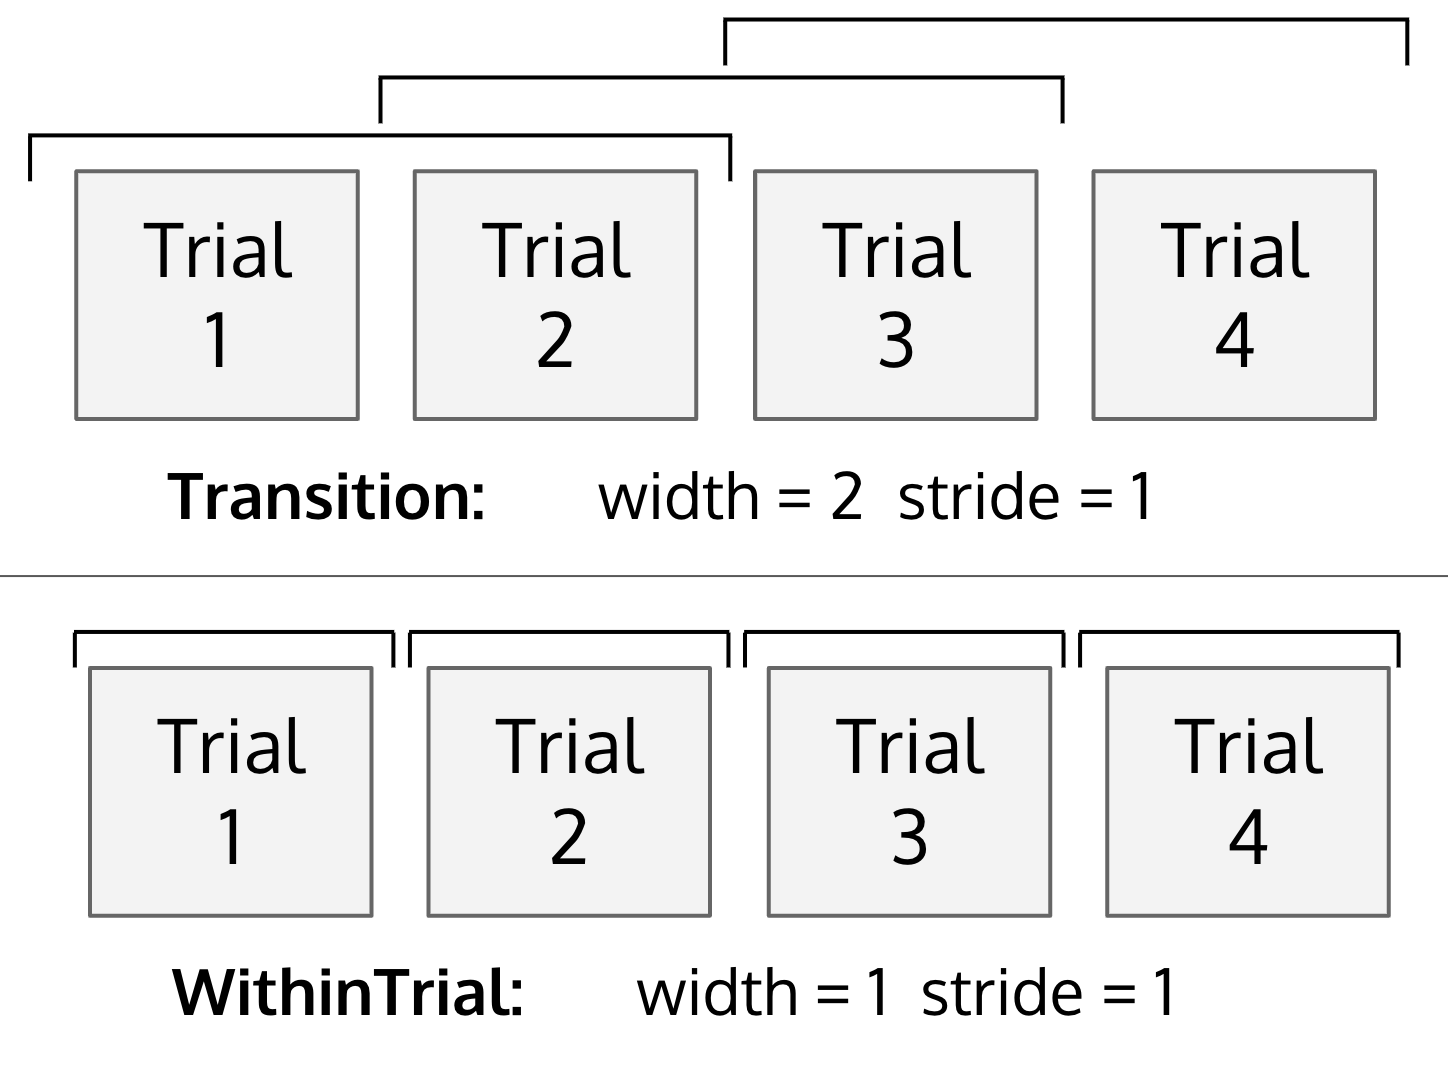
\includegraphics[origin=c,width=8cm]{../figures/windows.png}}
\caption{Window Properties}
\label{fig:windows}
\end{figure}

A second window alias exists, \texttt{Transition}, which has a width of two and a stride of one. As its name implies, this type of window is useful for expressing relationships between consecutive trials in a sequence. For example, a \texttt{Transition} window could be used to define a factor that determines if the level for \texttt{color} is repeated or not between two trials as follows:

\begin{verbatim}
def repeat(colors):
    return colors[0] == colors[1]

def switch(colors):
    return not repeat(colors)

color_repeats = Factor("Color Repetition", [
  DerivedLevel("Repeat",    Transition(repeat, [color])),
  DerivedLevel("No Repeat", Transition(switch, [color]))
])
\end{verbatim}

Observe that derived factors with this type of window never apply to the first trial in a sequence, as no prior trial exists with which to compare the current trial. Windows with non-one width and stride will not have a value for every trial in the sequence. Generally speaking, a window with width $w$ and stride $s$ will first apply to trial $w$, and to every $s^{th}$ trial after that. Although the language does allow for windows with arbitrary widths and strides, the computational complexity of computing the levels grows exponentially as the width increases. Therefore there are practical constraints on the usable size of a window.

\subsection{Crossing}

Once the user has defined some factors, a trial sequence could be generated by randomly combining different levels from each factor, but this would be insufficient. Researchers most often need to counterbalance or cross the levels of some factors to ensure that some particular combination of levels is present in the final sequence. The block specifies a subset of factors that should be used to construct this \textit{crossing}. The crossing is the cartesian product of the set of levels from each factor in the subset. For example, suppose two factors are selected to form the crossing, each with two levels: \texttt{[a, b]} and \texttt{[1, 2]}. The resultant crossing would be \texttt{[a, 1]}, \texttt{[a, 2]}, \texttt{[b, 1]}, and \texttt{[b, 2]}.

The crossing is the most authoritative constraint in the entire design. Every level combination in the crossing is required to be present in any generated trial sequence. Furthermore, a generated trial sequence will always have the minimum number of trials required to give full representation to the crossing. If there are $n$ level combinations in the crossing, then there must be at least $n$ trials in any generated trial sequence. If the crossing includes derived factors that span two or more trials (window width greater than one), then the minimum number of trials increases. For example, if the crossing contains a derived factor with a transition window, then generated trial sequences must have $n+1$ trials because the derived factor will not have a value in the first trial.

\subsection{Constraints}

Lastly, constraints allow the designer to require or prohibit particular patterns in the final generated trial sequence. There are only two such constraints available today: \texttt{AtMostKInARow} and \texttt{ExactlyKInARow}. Each of these allows the designer to enforce that there are no more than, or exactly, $k$ (user-specified) repetitions of a specific factor level in any generated sequence. These constraints are useful for ensuring some level of variety, or lack thereof, between trials in the sequence.

\subsection{Complete Example}

Having introduced each component of the block that defines a design, we can now view an example in full. This example will show how the Stroop test \cite{stroop1935studies}, a popular design among experimental psychologists, can be expressed in the SweetPea language. In the Stroop test, a subject perceives potential conflicts in the trial sequence that influence their reaction time. For example, a subject may be shown printed words representing colors and asked to read the word. However, the ink color of the word may be different from the printed word itself, leading to a delayed reaction due to the cognitive conflict. This design is easily represented in SweetPea as follows:

\begin{verbatim}
color = Factor("color", ["red", "green", "blue"])
text  = Factor("text",  ["red", "green", "blue"])

congruent = Factor("congruent?", [
    DerivedLevel("yes", WithinTrial(operator.eq, [color, text])),
    DerivedLevel("no",  WithinTrial(operator.ne, [color, text]))
])

constraints = [AtMostKInARow(1, ("congruent?", "yes"))]

block = FullyCrossBlock([color, text, congruent],
                        [color, text],
                        constraints)
\end{verbatim}

\texttt{color} and \texttt{text} represent the possibilities for the font color and the printed text in a trial. A \texttt{congruent} factor is also defined, to define a constraint that will ensure the subject never sees two consecutive trials in which the ink color and printed text matched. Lastly, the final block is constructed using just \texttt{color} and \texttt{text} to form the crossing. Table \ref{tab:example_sequence} shows one possible trial sequence that conforms to this design.

\begin{table}[htb]
  \centering
  \caption{Example Trial Sequence}
\begin{tabular}{cccc}
Trial & Color & Text  & Congruent \\
1     & blue  & green & no        \\
2     & red   & red   & yes       \\
3     & blue  & red   & no        \\
4     & green & red   & no        \\
5     & green & blue  & no        \\
6     & blue  & blue  & yes       \\
7     & red   & blue  & no        \\
8     & red   & green & no        \\
9     & green & green & yes
\end{tabular}
\label{tab:example_sequence}
\end{table}


\section{Current Implementation}

SweetPea encodes the experimental design in a boolean satisfiability (also known as SAT) formula such that any satisfying assignment represents a unique trial sequence that upholds the design. The assignment can then be translated back into the original design language for use as stimuli. At present SweetPea employs a simple positional encoding. In this encoding, a distinct variable represents every level of every factor of every trial. A SAT sampler is then applied to the formula to generate approximately uniformly distributed solutions.

\subsection{Boolean Satisfiability}

The Boolean satisfiability problem (abbreviated SAT) is the problem of determining whether or not a Boolean formula can be satisfied, or be caused to evaluate to true, by a particular true or false assignment to each of its variables. If a Boolean formula can encode the problem at hand, then techniques from satisfiability theory may be applied to determine whether or not a solution exists to the problem, or to locate a particular solution. Many different SAT solvers exist which accept a Boolean formula as input, and output either a solution to the formula or indicate that the formula is \textit{unsatisfiable}.

A SAT formula contains some number of boolean variables and propositional logic clauses. A selection of true or false for each variable in the formula constitutes an \textit{assignment}. If a given assignment causes the entire formula to evaluate to true, then the formula is said to be \textit{satisfied} by that assignment, or more generally, the formula is \textit{satisfiable}. If no such assignment exists, the formula is said to be \textit{unsatisfiable}.

Tools for interacting with SAT formulas typically require the input formula to be in \textit{conjunctive normal form} (abbreviated CNF), which is a form of a Boolean formula with specific properties. A Boolean formula is in conjunctive normal form only when it meets three conditions: the entire formula must be a conjunction of clauses, each clause consists of an individual variable or a disjunction of variables, and the negation operator may only appear on individual variables, not entire clauses. Any Boolean formula may be expressed in conjunctive normal form, though converting an arbitrary formula to CNF usually requires growth in some dimension. SweetPea uses the Tseitin Transformation \cite{tseitin1983complexity} to do this conversion, which has the tightest known bounds on formula length, at the expense of allocating additional variables.

\subsection{Example Encoding}

Continuing with the example design for the Stroop test introduced previously, we will see how SweetPea generates the SAT encoding for this design. The sequence length, as determined by the crossing, is $9$. The current encoding scheme will allocate $9 \cdot 8 = 72$ variables to represent every level of every factor in each trial. Additional variables will be allocated to enforce other constraints, such as ensuring that each factor takes only one level in each trial, and requiring that each combination in the crossing be present in the sequence. The first step of the encoding can be visualized easily, as demonstrated in Table \ref{tab:encoding_diagram}.

\begin{table}[htb]
  \centering
  \caption{Example of an Encoding Diagram}
\begin{tabular}{|r|c|c|c|c|c|c|c|c|}
\hline
\multicolumn{1}{|l|}{}             & \multicolumn{3}{c|}{Color} & \multicolumn{3}{c|}{Text} & \multicolumn{2}{c|}{Congruent?} \\ \hline
\multicolumn{1}{|l|}{Trial Number} & Red    & Green    & Blue   & Red    & Green   & Blue   & Yes             & No            \\ \hline
1                                  & 1      & 2        & 3      & 4      & 5       & 6      & 7               & 8             \\ \hline
2                                  & 9      & 10       & 11     & 12     & 13      & 14     & 15              & 16            \\ \hline
3                                  & 17     & 18       & 19     & 20     & 21      & 22     & 23              & 24            \\ \hline
4                                  & 25     & 26       & 27     & 28     & 29      & 30     & 31              & 32            \\ \hline
5                                  & 33     & 34       & 35     & 36     & 37      & 38     & 39              & 40            \\ \hline
6                                  & 41     & 42       & 43     & 44     & 45      & 46     & 47              & 48            \\ \hline
7                                  & 49     & 50       & 51     & 52     & 53      & 54     & 55              & 56            \\ \hline
8                                  & 57     & 58       & 59     & 60     & 61      & 62     & 63              & 64            \\ \hline
9                                  & 65     & 66       & 67     & 68     & 69      & 70     & 71              & 72            \\ \hline
\end{tabular}
\label{tab:encoding_diagram}
\end{table}

In this encoding, if variable 68 is true, that corresponds to the level \texttt{red} being selected for the factor \texttt{text} in trial number 9. The encoding will also require variables 69 and 70 to be false in this case, as well as require variable 71 to be equivalent to 65. Once a solution is found, it is then decoded back into the original language of the design as a trial sequence. For more details concerning the current encoding scheme, refer to the original paper.

Once SweetPea generates the CNF encoding for a design, it applies a SAT sampler to the formula to generate some number of solutions. SAT samplers are similar to solvers, in that they produce satisfying assignments to a boolean formula; however, they guarantee some level of uniformity in the distribution of generated samples. Historically, SAT samplers could only provide strong uniformity guarantees for small formulas, but recent research shows some potential for improving the scalability of current sampling algorithms. SweetPea targets the SAT sampler \textit{UniGen}. SAT sampling will be discussed in further detail later on.

\subsection{One-to-One Correspondence}

In order for the uniformity guarantees of sampling tools to translate back into the problem space of the original experiment design, the encoding scheme must maintain a one-to-one relationship between formula solutions and distinct trial sequences. Without this relationship, it would be possible to uniformly sample solutions to the SAT formula while still introducing bias in the generated trial sequences. For example, if three SAT solutions yielded trial sequence $S_1$, while only one solution yielded trial sequence $S_2$, uniformly distributed solutions to the SAT formula would produce $S_1$ more frequently than $S_2$.

A few observations build our confidence the encoding upholds this correspondence. First, all factor and level selections, including associated constraints for derived levels, in the original problem space are represented directly in the SAT encoding. A unique variable represents every level of every factor for every trial in the sequence. Clauses are added to the formula to ensure that variable assignments are consistent with the actual constraints of the problem. Referring back to the example in Table \ref{tab:encoding_diagram}, the levels for the \texttt{Color} factor for trial number 1 are represented by variables 1, 2, and 3 respectively. The SAT formula embeds a popcount, or Hamming weight, circuit that requires that exactly one of those variables be true. The encoding repeats this circuit for each of the nine trials for every factor. Other constraints are also embedded to represent all other rules of the design. Thes constraints enforce relationships between basic and derived factors, as well as guarantee that the full spectrum of crossed factor combinations appears in the sequence. Because SweetPea directly translates all data from the original design into SAT variables and constraints, we believe there is no risk of generating multiple solutions to the formula that represent the same trial sequence.

However, some of these constraints are represented using operators prohibited in CNF, including logical implication. Of necessity, these expressions must be rewritten in an equivalent form using only those primitives allowed by CNF. In order to avoid an exponential explosion in the length of the formula, this rewriting process introduces additional variables to represent repeating clauses. The second observation is that SweetPea applies the Tseitin transformation to do this conversion to CNF, which binds every variable that it introduces to the state of a clause in the original formula. As a result, the number of solutions remains the same, and there is no possibility of underconstrained variables skewing the results.

Lastly, we observe that for small designs, we can exhaustively enumerate all possible trial sequences. The number of enumerated sequences matches precisely the result obtained when using a SAT model counter to determine the number of solutions to the SAT formula. Were there not a one-to-one mapping, these figures would disagree.


\section{SweetPea's Contributions}

SweetPea was created to solve two specific problems facing researchers today:

\begin{enumerate}
\item No standard tooling exists for defining experimental designs. Researchers work independently to construct trial sequences for their designs using whatever means they deem appropriate. As a result, it is nearly impossible for researchers to collaborate and share their designs.
\item Trial sequences generated by researchers today are biased. Because they do not have sufficient tooling to sample trial sequences from a uniform distribution randomly, homebrew solutions make random choices with backtracking when constraint violations are detected. This approach skews the distribution of generated samples, making it difficult for peers to reproduce published results.
  \end{enumerate}

SweetPea aims to solve both of these problems by providing a standard language for expressing experimental designs as well as a synthesis engine that generates a uniform distribution of random samples.


\section{Conclusion}

SweetPea sounds panacean, but it has yet to realize its objectives fully. The language is still under revision, but SweetPea shows excellent promise for fulfilling the first objective. On the other hand, uniform sampling of trial sequences has proven significantly more challenging. We hoped that leveraging recent developments in the field of SAT-sampling would allow us to solve this problem. However, the applicability of SAT samplers is fundamentally limited to formulas with solution counts below a particular threshold. Realistic designs routinely exceed this threshold.

A solution to the formula represents a unique trial sequence in the design. Therefore every possible sequence permutation (so long as it upholds the design constraints) is also a distinct solution. Consequentially, the number of solutions grows factorially in the sequence length. In the previous example, the sequence length denoted $l$, was $9$. Without the congruence constraint, there would be $9! = 362,880$ solutions, which is still rather modest. Consider an experiment however in which $l = 36$. The solution count grows to $36! \approx 2^{138}$, which is many orders of magnitude larger. Table \ref{tab:factorial_explosion} shows how the number of solutions explodes as $l$ increases. As will be seen later, it is common for experimental designs to have sequence lengths even larger than 36.

\begin{table}[htb]
  \centering
  \caption{Growth of Solution Space}
\begin{tabular}{|l|r|}
\hline
\multicolumn{1}{|c|}{\textbf{Sequence Length ($l$)}} & \multicolumn{1}{c|}{\textbf{\#SAT ($l!$)}}              \\ \hline
4                                                    & 24                                                      \\ \hline
6                                                    & 720                                                     \\ \hline
9                                                    & 362,880                                                 \\ \hline
12                                                   & 479,001,600                                             \\ \hline
16                                                   & 20,922,789,888,000                                      \\ \hline
20                                                   & 2,432,902,008,176,640,000                               \\ \hline
25                                                   & 15,511,210,043,330,985,984,000,000                      \\ \hline
30                                                   & 265,252,859,812,191,058,636,308,480,000,000             \\ \hline
36                                                   & 371,993,326,789,901,217,467,999,448,150,835,200,000,000 \\ \hline
\end{tabular}
\label{tab:factorial_explosion}
\end{table}

In practice, designs have constraints; however, the constraints only exclude specific patterns in the permutations; therefore, the number of solutions remains dominated by $l!$. Furthermore, designs commonly contain several unconstrained factors, which magnifies the combinatorial explosion. Generating all possible solutions is not feasible.

It has been well established that prior SAT-samplers have traded strong uniformity guarantees for scalability \cite{chakraborty_balancing_2014}, and thus were not suitable for even moderately sized formulas. Unigen \cite{chakraborty_balancing_2014} contributed two primary advancements to bridge this gap between scalability and uniformity guarantees, but these advancements require specific conditions that impose fundamental limits on the number of possible solutions to the formula. This paper shows that experimental designs generally do not uphold these conditions, and therefore SAT samplers on their own are insufficient for generating uniformly distributed solutions. However, due to the combinatorial nature of these designs, arithmetic principles can be applied to directly construct uniformly distributed samples for some classes of experimental designs. Further success will likely involve a hybrid between sampling and construction approaches.
